\renewcommand{\nomebreve}{pacman}
\renewcommand{\titolo}{Percorsi tra pillole e fantasmi}

\introduzione{}

Tutti sanno che il giallo pacman è un tipo tranquillo che pensa solo a percorrere la propria strada. Quando pacman si imbatte in un fantasmino si disintegra con un'odiosa e pregnante musichetta che tutti conosciamo: per lui è game over e non potrà più completare il suo percorso. Ma sul campo di gioco sono cosparsi dei pillolazzi che donano a pacman un superpotere: quando pacman ne raccoglie uno esso gli assicura protezione per un certo intervallo di tempo di emancipazione e riscatto. Quando pacman è sotto l'effetto di qualche pillolazzo il suo colore, da giallo, è diventato blu, ed ora sono i fantasmi a doverlo temere!

\hspace{0.8cm}

\includegraphics[width=0.1\textwidth]{figures/pacman_big.png}
\hfill
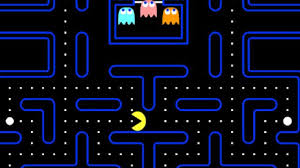
\includegraphics[width=0.22\textwidth]{figures/pacman_field.jpeg}
\hfill

\includegraphics[width=0.22\textwidth]{figures/pacman_rage.png}


Un pacman si muove su una griglia rettangolare di dimensioni $M\times N$.
Parte sereno e giallo, dalla cella $(1,1)$ in alto a sinistra, e deve raggiungere la cella $(M,N)$ in basso a destra.
Per farlo ha due tipi di mosse da considerarsi valide purch\`e non portino pacman fuori dalla griglia:
\begin{itemize}
   \item[] {\bf verso destra:} dalla cella $(i,j)$ alla cella $(i+1,j)$;
   \item[] {\bf verso il basso:} dalla cella $(i,j)$ alla cella $(i,j+1)$.
\end{itemize}

Ogni cella della griglia è contrassegnata da un carattere che ne specifica la tipologia come da seguente tabella:
\begin{itemize}
   \item['\#'] cella muro, resterà sempre inaccessibile a pacman;
   \item['+'] cella libera, pacman può visitarla liberamente;
   \item['*'] cella fantasma. Se pacman è blu quando ci arriva allora è lui che si pappa il fantasmino e può tranquillamente proseguire il proprio percorso come se nulla fosse successo. In caso contrario è game over, il percorso fin quì compiuto non è valido.
   \item[n] quì $n$ è un numero naturale compreso tra $1$ e $5$. Siamo in una cella pillolazzo. Quando pacman dovesse transitare per questa cella si assicura di essere di colore blu nelle prossime $n$ celle che andrà a visitare. Il colore blu stà ad indicare che pacman è incazzato nero (rage), un po' come quando ad Hulk gli sale il verde e diventa invincibile. A differenza dell'incredibile Hulk, pacman non perde mai il controllo e continua a rispettare i muri.
\end{itemize}

La domanda \`e quanti siano i percorsi validi possibili.
Per non introdurre le difficolt\`a meramente tecniche della gestione di numeri arbitrariamente grandi, vi chiedo di restituire solamente le ultime sei cifre decimali della risposta, ossia il numero di percorsi modulo $1\,000\,000$ (eventuali zeri iniziali vanno quindi omessi).

\section*{Dati di input}
Il programma legge da un file di nome \file{input.txt}. La prima riga contiene due interi positivi $M$ ed $N$, separati da spazio, i quali rappresentano le dimensioni della scacchiera.
Le successive $M$ righe rappresentano la mappa: la $r$-esima di tali righe contiene una
sequenza di $N$ caratteri nell'alfabeto $\{+,\#,*,1,2,3,4,5\}$, il cui significato è stato specificato più sopra.
Ovviamente, il $c$-esimo carattere di questa riga si riferisce alla cella $(r, c)$ della mappa. I caratteri NON sono separati da spazi.

Tenete presente che ci saranno i caratteri di terminazione di riga. (Potete avvalervi del template di soluzione fornito in attachment alla pagina del problema per gestire in modo robusto queste piccole noie). 

\section*{Dati di output}
Il programma deve scrivere in un file di nome \file{output.txt}. Deve venire stampato un unico numero, il numero di percorsi (modulo $1\, 000\, 000$) che PacMan può seguire per arrivare da cella $(1,1)$ a cella $(M,N)$.


% Esempi
\section*{Esempio di input/output}

In attachment alla pagina del problema trovate diverse copie input/output tra cui le seguenti.

\vspace{0.5cm}
\esempio{
5 4

+5+2

\#+2+

+\#++

\#\#+*

\#\#++

}{9}

\esempio{
3 5

+41++

\#+3+*

+\#**+

}{8}

\section*{Assunzioni}
\begin{itemize}
\item pacman nasce giallo nella cella $(1, 1)$, una cella sgombra da fantasmi e non di muro
\item $0 < M,N \le 500$
\end{itemize}

\section*{Subtask}
\begin{itemize}
\item \textbf{Subtask 1 [0 punti]:} casi di esempio (inclusi quelli in attachment).
\item \textbf{Subtask 2 [10 punti]:} senza fantasmi, $M,N \le 10$.
\item \textbf{Subtask 3 [10 punti]:} senza pillolazzi, $M,N \le 10$.
\item \textbf{Subtask 4 [10 punti]:} senza fantasmi.
\item \textbf{Subtask 5 [10 punti]:} senza pillolazzi.
\item \textbf{Subtask 6 [20 punti]:} $M,N \le 10$.
\item \textbf{Subtask 8 [20 punti]:} $M,N \le 100$.
\item \textbf{Subtask 9 [20 punti]:} nessuna restrizione, $M,N \le 500$.
\end{itemize}

\end{document}

